\clearpage
\section{Oblivious Transfer with Discrete Variables}

\begin{tcolorbox}	
\begin{tabular}{p{2.75cm} p{0.2cm} p{10.5cm}} 	
\textbf{Student Name}  &:& Mariana Ramos\\
\textbf{Starting Date} &:& September 18, 2017\\
\textbf{Goal}          &:& Oblivious transfer implementation with discrete variables.
\end{tabular}
\end{tcolorbox}

Oblivious Transfer (OT) is a fundamental primitive in multi-party computation. The one-out-of-two OT consists in a communication protocol between Alice and Bob. At the beginning of the protocol Alice has two messages $m_1$ and $m_2$ and Bob wants to know one of them, $m_b$, without Alice knowing which one, i.e. without Alice knowing $b$, and Alice wants to keep the other message private, i.e. without Bob knowing $m_{\bar{b}}$. therefore two conditions must be fulfilled:
\begin{enumerate}
	\item{The protocol must be concealing, i.e at the beginning of the protocol Bob does not know nothing about Alice's messages, while at the end of the protocol Bob will learn the message $m_{b}$ chosen by him.}
	\item{The protocol is oblivious, i.e Alice cannot learn anything about Bob's choice, bit $b$, and Bob cannot learning nothing about the other message $m_{\bar{b}}$.}
\end {enumerate}

\subsection{OT Protocol Detailed}
In this section, we are going to detail an 1-out-2 OT Protocol's implementation using discrete variables and single photon polarization encoding.

 First of all, it is important to set the initial conditions of Bob and Alice's knowledge.

In general, the first step is to establish for both Alice and Bob the message length $s$ and the parameter $k$, which is an expansion factor of message's length.
In this case, lets assume message's length $s=4$ and an expansion factor $k=2$.

 In addition, both Alice and Bob know the following correspondence, where $+$ corresponds to \textit{Rectilinear Basis} and $\times$ corresponds to \textit{Diagonal Basis}:

\begin{table}[H]
\centering
\begin{tabular}{c|c}
\textbf{\textit{Basis}}         &  \\ \hline
 0 & $+$ \\
 1 & $\times$ \\
\end{tabular}
\end{table}

Secondly both Alice and Bob also know the bit correspondence for each direction for each basis. For \textit{Rectilinear basis}, "$+$":

\begin{table}[H]
\centering
\begin{tabular}{c|c}
            & Basis "+" \\ \hline
 0 & $\to (0^{\circ})$ \\
 1 & $\uparrow (90^{\circ})$ \\
\end{tabular}
\end{table}

and for \textit{Diagonal Basis}, "$\times$":

\begin{table}[H]
\centering
\begin{tabular}{c|c}
      & Basis "$\times$" \\ \hline
 0 & $\searrow (-45^{\circ})$ \\
 1 & $\nearrow (45^{\circ})$ \\
\end{tabular}
\end{table}

Third, only Alice knows information about messages $m_{0}$ and $m_{1}$.
In this case, lets assume she sets the two messages $m_{0} = \{0 0 1 1\}$ and $m_{1} = \{0 0 0 1\}$.

\begin{enumerate}
  \item Alice randomly generate a bit sequence with length $ks$ being, in this case, $k=2$ and $s=4$ as it was defined at the beginning.
      Therefore, she must define two sets randomly: $S_{A1}$ which contains the basis values; and $S_{A2}$, which contains the key values.

      In that case, lets assume she gets the following sets $S_{A1}$ and $S_{A2}$:
      $$S_{A1} = \{0,1,1,0,0,1,0,1 \},$$
      $$S_{A2} = \{1,1,0,0,0,1,0,0 \}.$$

  \item Next, Alice sends to Bob throughout a quantum channel $ks$ photons encrypted using the basis defined in $S_{A1}$ and according to the keys defined in $S_{A2}$.

      In the current example, Alice sends the photons, throughout a quantum channel, according to the following,

      $$S_{AB} = \{\uparrow, \nearrow, \searrow, \to, \to, \nearrow, \to, \searrow \}.$$
       $$S_{AB} = \{90^{\circ}, 45^{\circ}, -45^{\circ}, 0^{\circ}, 0^{\circ}, 45^{\circ}, 0^{\circ}, -45^{\circ} \}.$$

  \item Bob also randomly generates $ks$ bits, which are going to define his measurement basis, $S_{B1}$. He will measure the photons sent by Alice. Lets assume:

  $$S_{B1} = \{0,1,0,1,0,1,1,1 \}.$$

    When Bob receives photons from Alice, he measures them using the basis defined in $S_{B1}$.
  In the current example, $S_{B1}$ corresponds to the following set:
  $$\{ +,\times,+,\times,+,\times, \times, \times \}.$$
  Bob will get $ks$ results:
  $$S_{B1'} = \{1,1,0,1,0,1,1,0 \}.$$

  \item Bob will send a \textit{Hash Function} result HASH1 to Alice. This value will do Bob's commitment with the measurements done. In this case, this \textit{Hash Function} is calculated from \textit{SHA-256} algorithm for each pair (Basis from $S_{B1}$ and measured value from $S_{B1'}$), i.e Bob sends to Alice $sk$ pairs as his commitment. In this case, Bob sends eight pairs encoded using a \textit{Hash Function} which is also send to Alice. From that moment on Bob cannot change his commitment neither the basis which he uses to measure the photons sent by Alice.

  \item Once Alice has received the confirmation of measurement from Bob, she sends throughout a classical channel the basis which she has used to codify the photons, which in this case we assumed $S_{A1} = \{0,1,1,0,0,1,0,1\}$.

  \item In order to know which photons were measured correctly, Bob does the operation $S_{B2}=S_{B1} \oplus S_{A1}$.
      In the current example the operation will be:

  \begin{table}[H]
    \centering
    \begin{tabular}{c|c c c c c c c c}
     $S_{B1}$ & 0 & 1 & 0 & 1 & 0 & 1 & 1 & 1 \\
     $S_{A1}$ & 0 & 1 & 1 & 0 & 0 & 1 & 0 & 1 \\ \hline
     $\oplus$ & 1 & 1 & 0 & 0 & 1 & 1 & 0 & 1
    \end{tabular}
    \end{table}

      In this way, Bob gets $$S_{B2} = \{1,1,0,0,1,1,0,1 \}.$$ When Bob uses the right basis he gets the values correctly, when he uses the wrong basis he just guess the value. The values ``$1$'' correspond to the values he measured correctly and ``$0$'' to the values he just guessed.

       Next, Bob sends to Alice, through a classical channel, information about the minimum number between ``ones'' and ``zeros'', i.e $$n=min(\#0,\#1)=3,$$ where $\#0$ represents the number of zeros in $S_{B2}$ and $\#1$ the number of ones in $S_{B2}$. At this time, Alice must be able to know if Bob is being honest or not. Therefore, she will open Bob's commitment from \textit{step 4} and she verify if the number n sent by Bob is according with the commitment values sent by him. In other words, she opens a number of pairs committed by Bob which is known from the beginning. 

  \item If $n<s$, being \textit{s} the message's size, Alice and Bob will repeat the steps from $1$ to $7$. In this case, $n=3$ which is smaller than $s=4$. Therefore, Alice and Bob repeat the steps from 1 to 7 in order to enlarge Bob's sets $S_{B1}$ and $S_{B2}$ as well as Alice's sets $S_{A1}$ and $S_{A2}$.

  \item Lets assume :

   $$S_{B1}= \{1,1,0,0,0,1,0,0,1,0,0,0,0,0,1,1 \}.$$

    At Alice's side the new sets $S_{A1}$, which contains the basis values, and $S_{A2}$, which contains the key values, will be the following:

    $$S_{A1}=\{0,1,1,0,0,1,0,1,1,1,0,0,1,1,1,0 \},$$ $$S_{A2}=\{1,1,0,0,0,1,0,0,1,0,1,0,0,0,1,1 \}.$$

    Finally, for $S_{B2}=S_{B1} \oplus S_{A1}$ Bob gets the following sequence:

    $$S_{B2}= \{1,1,0,0,1,1,0,1,0,1,0,0,1,1,0,1 \}.$$

    Note that the sets were enlarge in the second iteration.

  \item At this time, Bob sends again to Alice, through a classical channel, the minimum number between  ``ones'' and ``zeros'',  $n=min(\#0,\#1)$. In this case, $n$ is equal to $7$ which is the number of zeros.

  \item Alice checks if $n>s$ and acknowledge to Bob that she already knows that $n>s$. In this case, $n=7$ and $s=4$ being $n>s$ a valid condition.

  \item Next, Bob defines two new sub-sets, $I_{0}$ and $I_{1}$. $I_{0}$ is a set of values with photons array positions which Bob just guessed the measurement since he did not measure them with the same basis as Alice, $I_{1}$ is a set of values with photons array positions which Bob measured correctly since he used the same basis as Alice used to encoded them.

  In this example, Bob defines two sub-sets with size $s=4$:
  $$I_{0}=\{3,4,7,11 \},$$
  and $$I_{1}= \{2,5,6,13 \},$$ where $I_{0}$ is the sequence of positions in which Bob was wrong about basis measurement and $I_{1}$ is the sequence of positions in which Bob was right about basis measurement. Bob sends to Alice the set $S_{b}$

  Thus, if Bob wants to know $m_{0}$ he must send to Alice throughout a classical channel the set $S_{0}=\{I_{1},I_{0} \}$, otherwise if he wants to know $m_{1}$ he must send to Alice throughout a classical channel the set $S_{1}=\{I_{0},I_{1} \}$.


  \item With both the received set $S_{b}$ and the hash function value HASH1, Alice must be able to prove that Bob has being honest. 

  \item Lets assume Bob sent $S_{0}=\{I_{1},I_{0} \}$.
   Alice defines two encryption keys $K_{0}$ and $K_{1}$ using the values in positions defined by Bob in the set sent by him. In this example, lets assume: $$K_{0}=\{1,0,1,0\}$$ $$K_{1}=\{0,0,0,1\}.$$

   Alice does the following operations:
   $$m = \{m_{0}\oplus K_{0}, m_{1} \oplus K_{1} \}.$$

   \begin{table}[H]
    \centering
    \begin{tabular}{c|c c c c c c c c}
     $m_{0}$ & 0 & 0 & 1 & 1 \\
     $K_{0}$ & 1 & 0 & 1 & 0 \\ \hline
     $\oplus$ & 1 & 0 & 0 & 1
    \end{tabular}
    \end{table}

   \begin{table}[H]
    \centering
    \begin{tabular}{c|c c c c c c c c}
     $m_{1}$ & 0 & 0 & 0 & 1 \\
     $K_{1}$ & 0 & 0 & 0 & 1 \\ \hline
     $\oplus$ & 0 & 0 & 0 & 0
    \end{tabular}
    \end{table}

    Adding the two results, $m$ will be: $$m=\{1,0,0,1,0,0,0,0\}.$$

   After that, Alice sends to Bob the encrypted message $m$ through a classical channel.

  \item When Bob receives the message $m$, in the same way as Alice, Bob uses $S_{B1\prime}$ values of positions given by $I_{1}$ and $I_{0}$ and does the decrypted operation. In this case, he does following operation:

      \begin{table}[H]
        \centering
        \begin{tabular}{c|c c c c c c c c}
         $m$ & 1 & 0 & 0 & 1 & 0 & 0 & 0 & 0 \\
             & 1 & 0 & 1 & 0 & 0 & 1 & 1 & 0 \\ \hline
         $\oplus$ & 0 & 0 & 1 & 1 & 0 & 1 & 1 & 0 \\
        \end{tabular}
        \end{table}

      The first four bits corresponds to message 1 and he received $\{0,0,1,1\}$, which is the right message $m_{0}$ and $\{0,1,1,0\}$ which is a wrong message for $m_{1}$.


\end{enumerate}

\subsection{OT Protocol - Open Issues}
Steps $4$ and $12$ are not fully defined.
\begin{enumerate}
  \item In step $4$ Bob may says to Alice that he has already measured the photon and it could be a lie. In order to prevent this an Hash Function must be used.

  \item In step $12$ Bob may uses some values in a dishonest way, i.e Bob can pick values from $I_{1}$ which he knows they are correct and send them in $I_{0}$ in order to know correct information about message $m_{\bar{b}}$.
\end{enumerate}

This problems can hopefully be solved using \textit{Bit Commitment} through \textit{Hash Functions}.


\subsection{Simulation}

First of all, the protocol will be simulated and then a experimental setup will be built in the laboratory.

The main goal of this simulation is to demonstrate that Bob was able to learn correctly message $m_{b}$ and he does not know the message $m_{\overline{b}}$.

\begin{figure}[H]
	\centering
	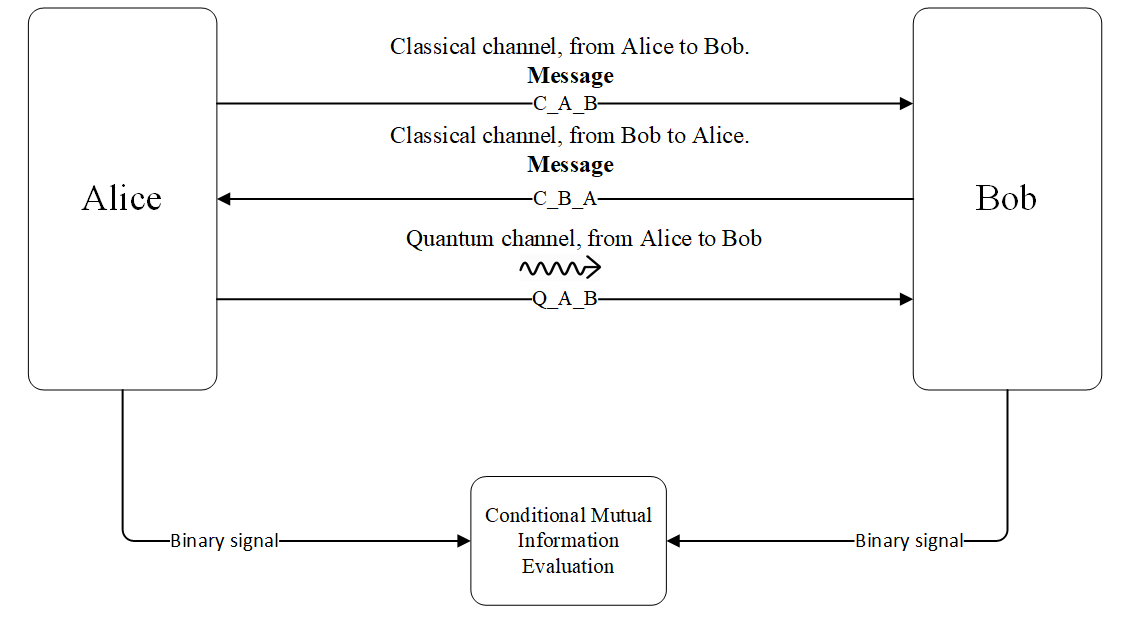
\includegraphics[width=1.0\textwidth, height=9cm]{./sdf/ot_with_discrete_variables/figures/Simulation_diagram_top.png}
	\caption{Simulation diagram at a top level}\label{toplevelsimulation}
\end{figure}

As one may see in figure \ref{toplevelsimulation} this simulation will have three top level blocks. Two of them are Alice and Bob and they are connected through two classical channels and one quantum channel. In addition, a third block will be performed in order to calculate the \textit{Mutual Information}. The mutual information (MI) between Alice and Bob is defined in terms of their join distribution.


\begin{enumerate}
  \item

  \begin{figure}[h]
	\centering
	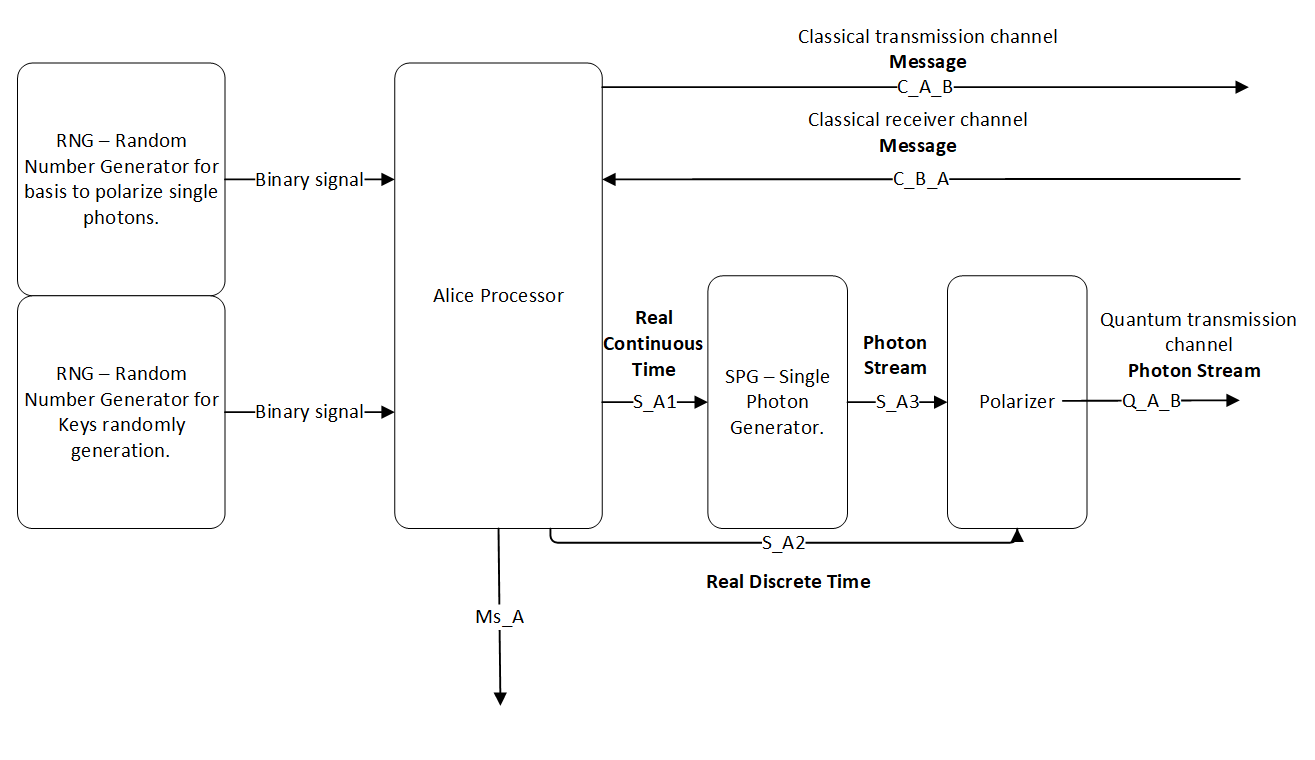
\includegraphics[width=1.1\textwidth, height=9cm]{./sdf/ot_with_discrete_variables/figures/Simulation_Alice.png}
	\caption{Simulation diagram - Alice's side}\label{simulationalice}
\end{figure}

    In figure \ref{simulationalice} one can observe a block diagram of the simulation at Alice's side. As it is shown in the figure, Alice must have two blocks for random number generation: one for basis generation in order to polarize the photons according this basis, and other for key random generation in order to have a random state to encode each photon. Furthermore, she has a Processor block for all logical operations: array analysis, hash function results validation, and others. This block also receives the start information, i.e. message size s, the expansion factor k and messages $m_{0}$ and $m_{1}$, as well as information from Bob, i.e sets $I_{0}$ and $I_{1}$, hash function results, and others. This block also must be responsible for send classical information to Bob. Finally, Processor block will also send a real continuous time signal to single photon generator, in order to generate photons according to this signal, and finally this block also sends to polarizer a real discrete signal in order to inform the polarizer which basis it should use. Therefore, she has two more blocks for quantum tasks: the single photon generator and the polarizer block which is responsible to encode the photons generated from the previous block and send them throughout a quantum channel from Alice to Bob.

    Finally, Alice's processor has an output to Mutual Information top level block, $Ms_{A}$.

  \item

  \begin{figure}[h]
	\centering
	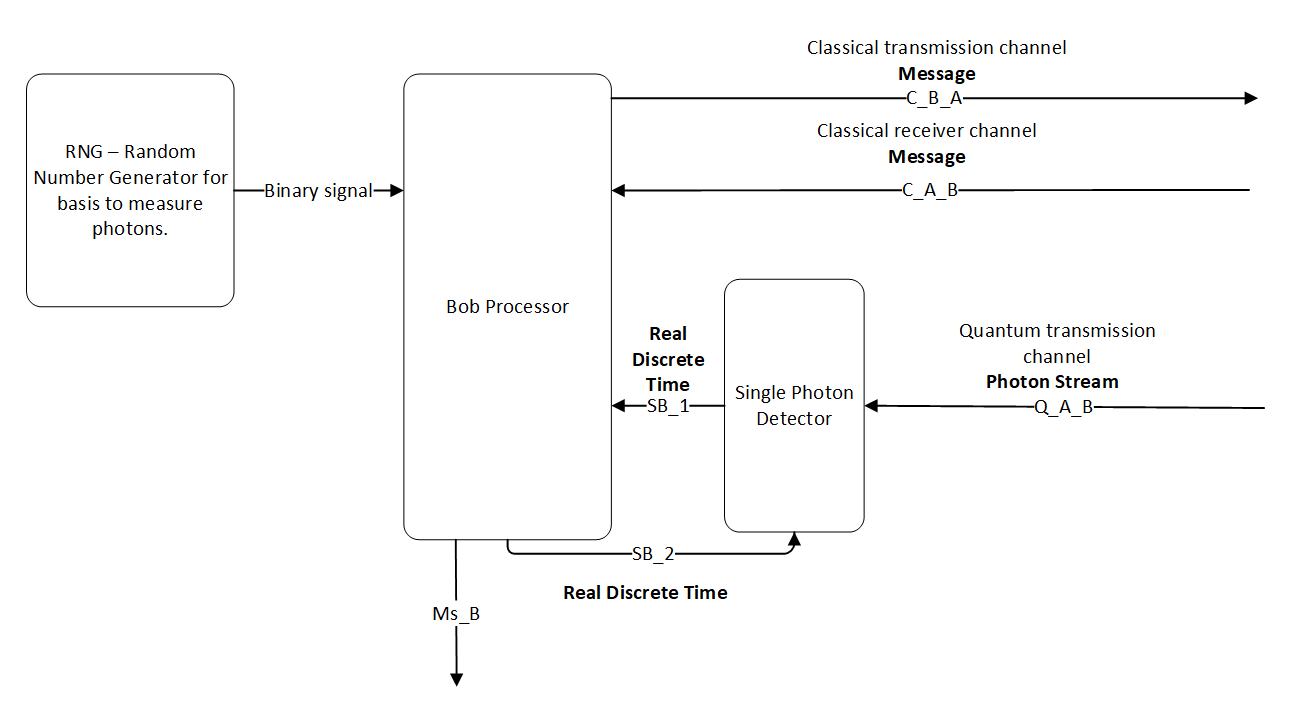
\includegraphics[width=1.1\textwidth, height=9cm]{./sdf/ot_with_discrete_variables/figures/Simulation_Bob.png}
	\caption{Simulation diagram - Bob's side}\label{simulationbob}
\end{figure}

    In figure \ref{simulationbob} one can observe a block diagram of the simulation at Bob's side. From this side, Bob only has one block for Random Number Generation which is responsible for randomly generate basis values which Bob will use to measure the photons sent by Alice throughout the quantum channel. Like Alice, Bob has a Processor block responsible for all logical tasks, i.e Hash function generation, analysing functions, etc. It receives information from Alice throughout a classical channel and a quantum channel but it sends information to Alice only throughout a classical channel. Furthermore, Bob has one more block for single photon detection which receives from processor block a real discrete time signal, in order to obtain the basis it should use to measure the photons.

    Finally, Bob's processor has an output to Mutual Information top level block, $Ms_{B}$.

  \item Mutual Information calculation
  \item
  \item
  \item
\end{enumerate}





\subsection{Experimental}
In figures \ref{quantumchannelcommunication1} and \ref{quantumchannelcommunication2} are presented the experimental setup to be performed in the lab. Starting with Alice's side and then Bob's side.

\begin{figure}[H]
	\centering 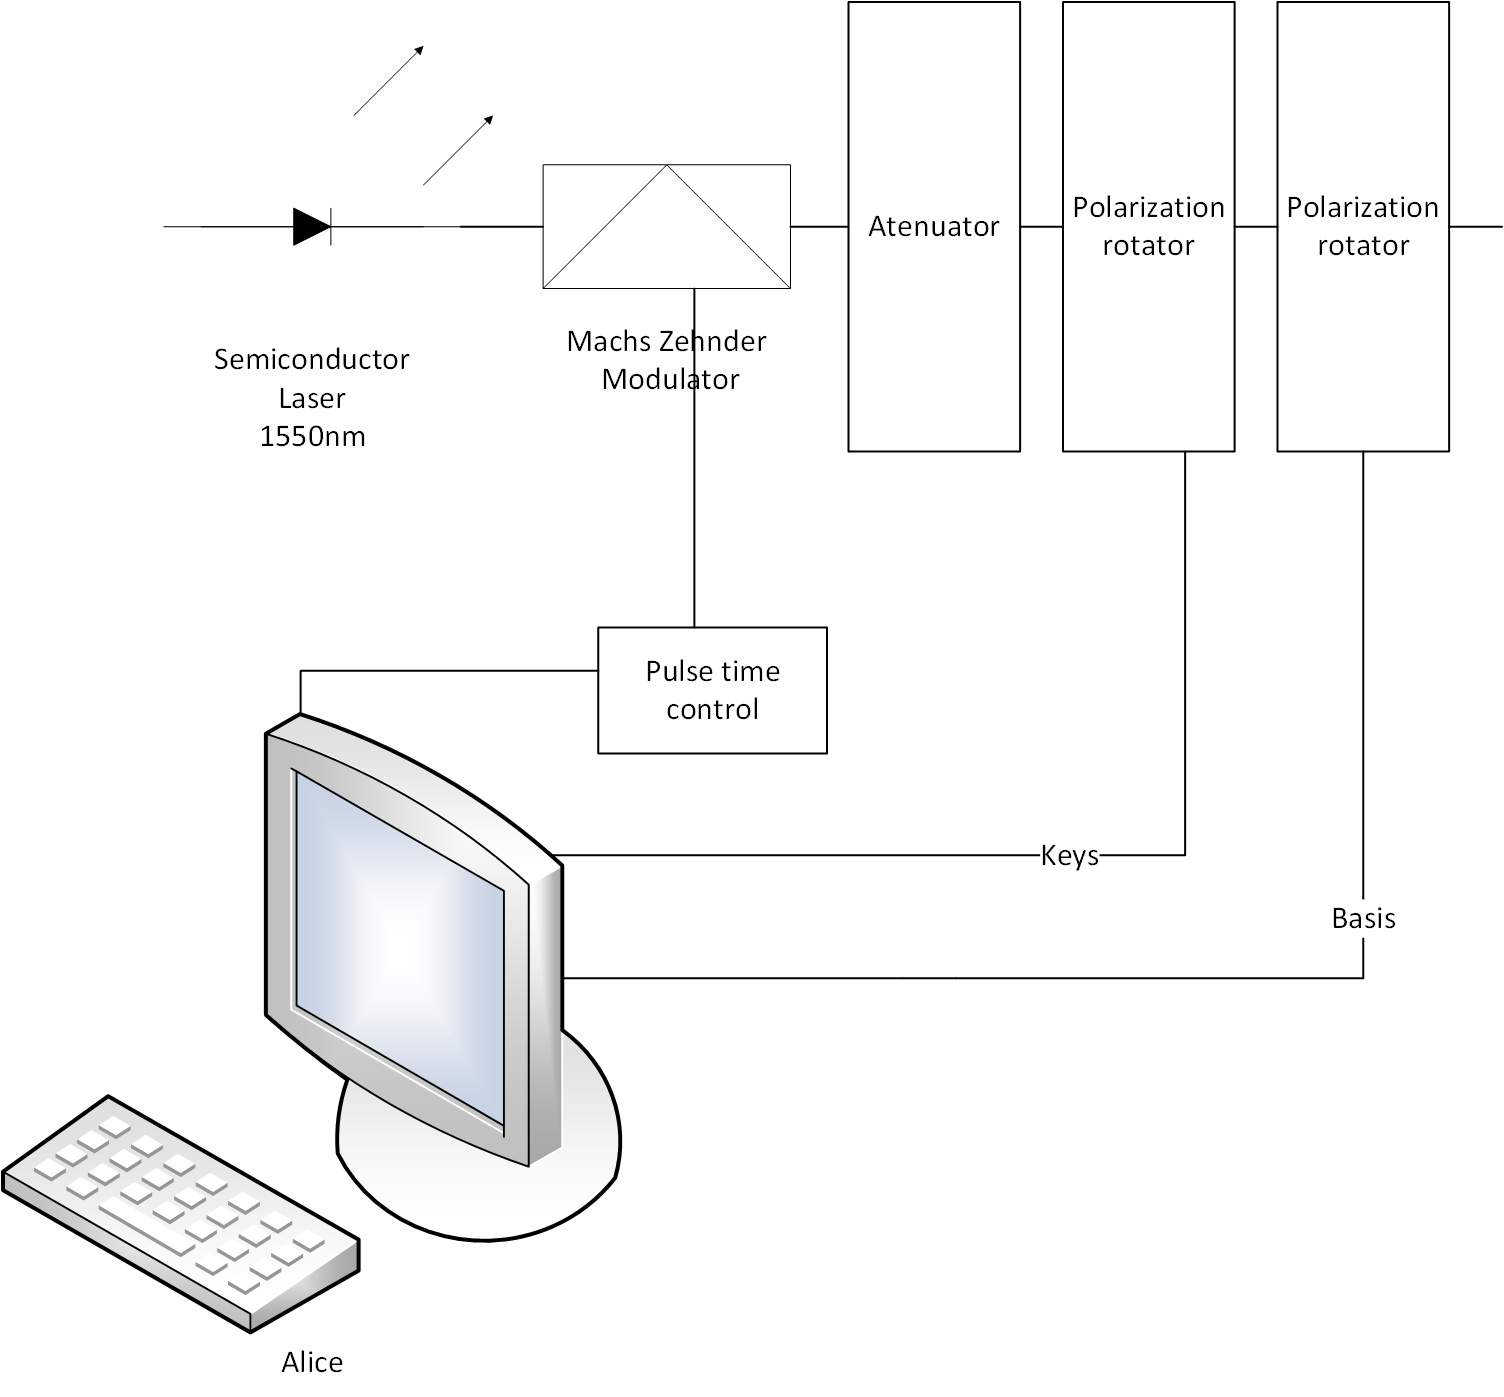
\includegraphics[width=0.8\textwidth,height=8cm]{./sdf/ot_with_discrete_variables/figures/OT_experimental_alice.png}
	\caption{Quantum communication diagram - Alice's side}\label{quantumchannelcommunication1}
\end{figure}

\begin{figure}[H]
	\centering 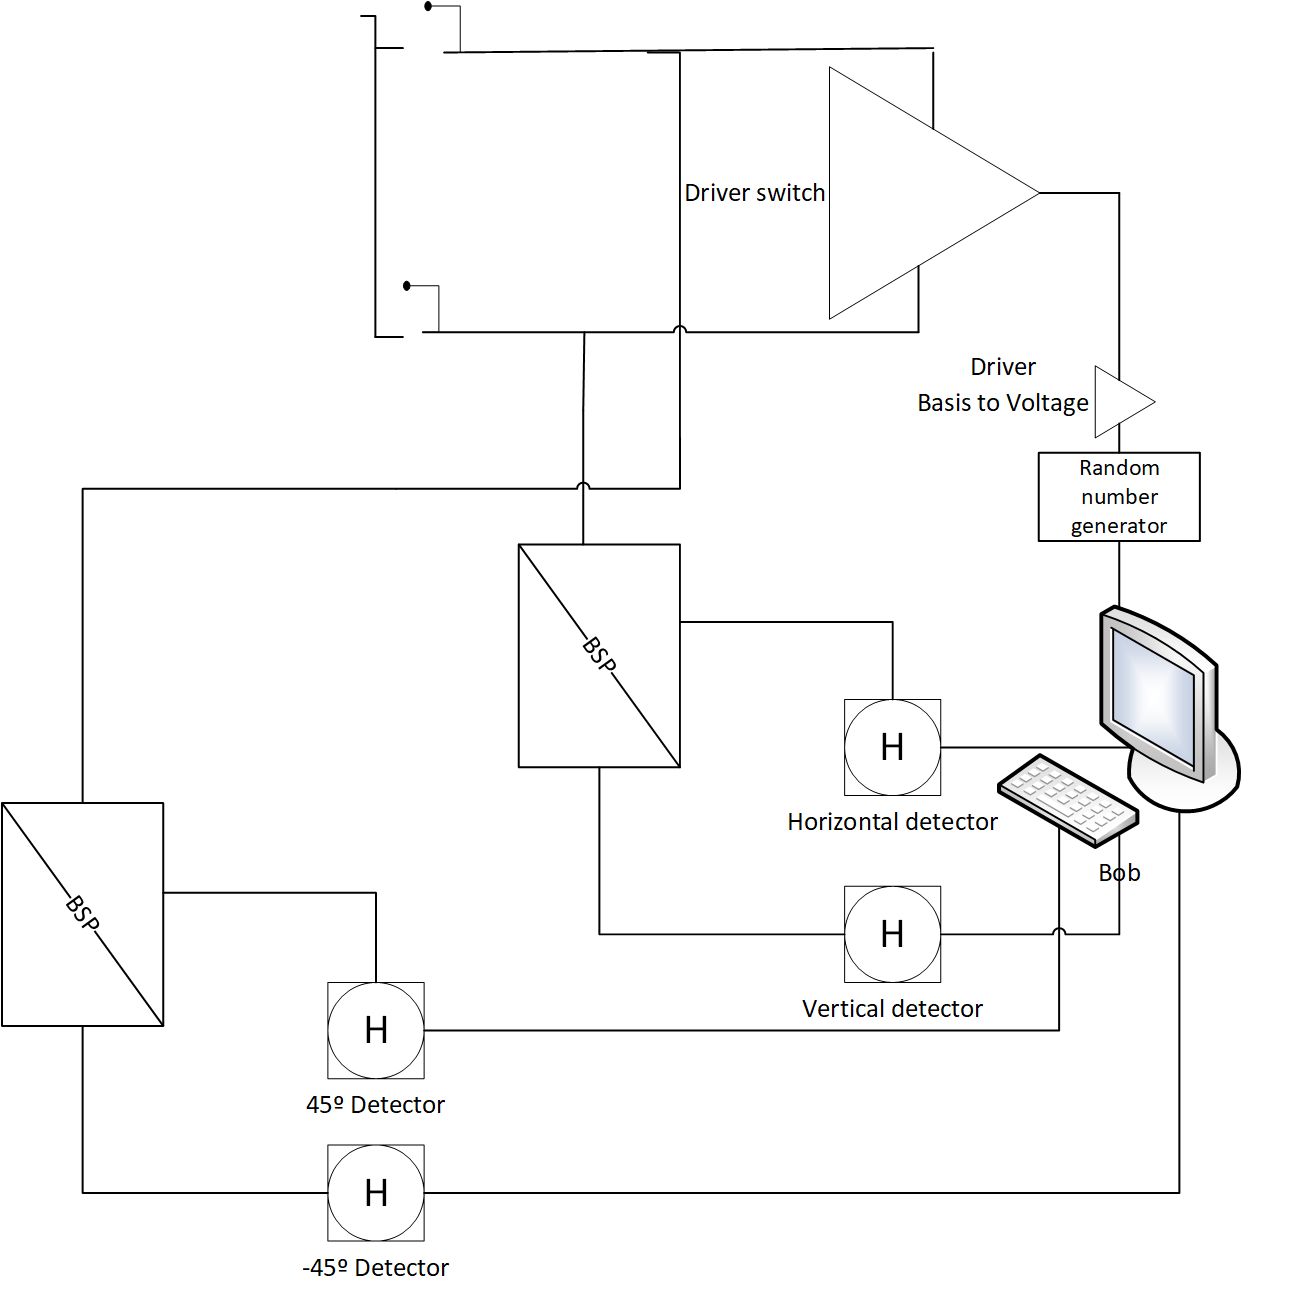
\includegraphics[width=0.8\textwidth,height=9cm]{./sdf/ot_with_discrete_variables/figures/OT_experimental_bob.png}
	\caption{Quantum communication diagram - Bob's side}\label{quantumchannelcommunication2}
\end{figure} 